\documentclass{article}
%
%
%	A Few Notes on Euler's Formula and Euler's Identity
%
%	David Meyer
%	dmm613@gmail.com
%	15 July 2022
%
%
%   get various packages
%
\usepackage[margin=1.0in]{geometry}                                     % adjust margins
\geometry{letterpaper}                                                  % or a4paper or a5paper or ... 
\usepackage{url}                                                        % need this to use URLs in bibtex
\usepackage{setspace}                                                   % need this for \setstrech{...}
\usepackage{scrextend}                                                  % need this for addmargin
\usepackage[export]{adjustbox}                                          % need this to get frame for includegraphics
%
%   tikz et al
%
\usepackage{tikz}
\usetikzlibrary{calc,patterns,angles,quotes,shapes,math,decorations,
                through,intersections,lindenmayersystems,backgrounds}
\usepackage{circuitikz}                                                 % draw circuits    
\usepackage{pgfplots}
\usepackage{pgfplots}	
%
%	more math stuff
%
\usepackage{amsmath,amsfonts,amssymb,amsthm}
\usepackage{mathtools}
\usepackage{commath}                                                    % get \norm{x}
\usepackage{fixmath}                                                    % get \mathbold
\usepackage{gensymb}                                                    % get \degree
\usepackage{mathrsfs}
\usepackage{hyperref}
\usepackage{subcaption}
\usepackage{authblk}
\usepackage{graphicx}
\usepackage{hyperref}
\usepackage{alltt}
\usepackage{color}
\usepackage{float}
\usepackage{braket}
\usepackage{siunitx}
\usepackage{relsize}
\usepackage{multirow}
\usepackage{esvect}
%
%	watermarks
%
% \usepackage{draftwatermark}
% \SetWatermarkText{Draft}
% \SetWatermarkScale{5}
% \SetWatermarkLightness {0.9} 
% \SetWatermarkColor[rgb]{0.7,0,0}
%
%
%	theorems, definitions, etc
%
\theoremstyle{definition}
\newtheorem{theorem}{Theorem}[section]
\newtheorem{definition}{Definition}[section]
\newtheorem{proposition}{Proposition}[section]
\newtheorem{lemma}{Lemma}[section]
\newtheorem{example}{Example}[section]
\newtheorem{remark}{Remark}[section]
%
%	The following code allows you to do
%
%	\begin{bmatrix}[r] (or [c] or [l])
%
\makeatletter
\renewcommand*\env@matrix[1][c]{\hskip -\arraycolsep
  \let\@ifnextchar\new@ifnextchar
  \array{*\c@MaxMatrixCols #1}}
\makeatother
%
%	make \arg{min,max}_{n \to \infty} work nicely
%
\newcommand{\argmax}{\operatornamewithlimits{argmax}}
\newcommand{\argmin}{\operatornamewithlimits{argmin}}
%
%	also a handy command
%
\newcommand*{\Scale}[2][4]{\scalebox{#1}{$#2$}}%
%
%	Title, author and date
%
\title{A Few Notes on Euler's Formula and Euler's Identity}
\author{David Meyer \\ \href{mailto:dmm613@gmail.com}
                            {dmm613@gmail.com}}
\date{Last Update: \today \\
	 {\vspace{1.00mm} \small Initial Version: May 17, 2020}}

%
%
\begin{document}
\maketitle
%
%
%
\bigskip
\section{Why does a complex number $z$ equal $r\mathrm{e}^{i \theta}$?}
Our first question regards the nature of a complex number $z$,
where the length of the line from the origin to the point $z$,
$|z|$, equals $r$.  In particular, why does a complex number
$z = a + bi = r \mathrm{e}^{i \theta}$?

\bigskip
\noindent
Well, consider the complex plane, shown in Figure \ref{fig:complex_plane}:

\bigskip
\begin{figure}[H]
\centering
  \resizebox{0.45 \textwidth}{!} {														% resize figure if you want
    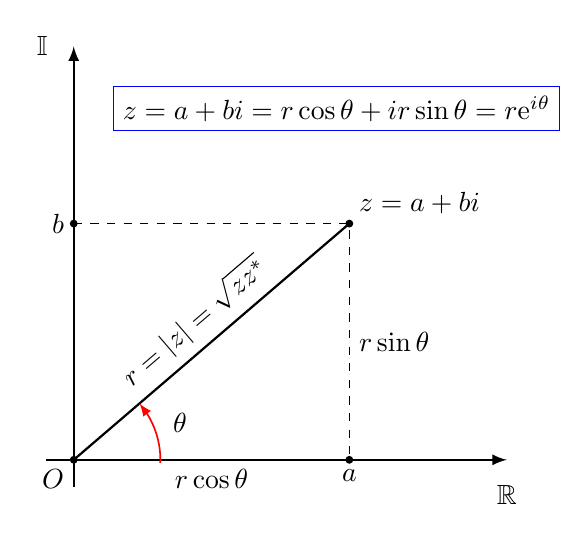
\begin{tikzpicture} [every edge quotes/.append style = {anchor=south, sloped}]
		\coordinate (O) at (0,0);														% name a coordinate for the origin
%
%	draw axes, saving the real part to calculate the angle (below)
%
		\draw[thick, -latex] (-0.35,0.00) -- (5.50,0.00) coordinate[yshift=-0.20cm,label=below: $\mathbb{R}$] (x);
		\draw[thick, -latex] (0.00,-0.35) -- (0.00,5.25) node[xshift=-0.2cm,left] {$\mathbb{I}$}
				node[draw,rectangle,thin,blue,below right=5.0mm]						%
            		{$\color{black}{													%
						z = a + bi = 													% z = <a bunch of stuff>
						r \cos \theta + i r \sin \theta = 								%
						r \mathrm{e}^{i\theta}}$};										%
		\coordinate[label=below left:$O$] (O);                                          % label origin
		\fill (O) circle(0.05);                                                         % draw a black dot at the origin
		\fill (3.5,3) coordinate[label=above right:{$z = a + bi $}] (z) circle(0.05);   % draw phasor and a dot (circle(0.05))
		\draw[dashed] (0,3) node[left] {$b$} -| (3.5,0) node[below] {$a$};              % draw dashed lines to a and b
		\draw [draw=none] (0,0) -- (3.5,0) node [midway, below]{${r \cos \theta}$};     % use [draw=none] to put label midway
		\draw [draw=none] (3.5,3.0) -- (3.5,0) node [midway, right]{${r \sin \theta}$};	% use [draw=none] to put label midway
		\fill (0,3) circle(0.05);                                                       % draw a dot on the y axis at b 
		\fill (3.5,0) circle(0.05);                                                     % draw a dot on the y axis at a
		\draw[thick] (O) to ["$r = |z|=\sqrt{zz^*}$"] (3.5,3);                          % label r
		\pic [draw=red, line width=0.60pt, -latex , angle radius=11mm,                  % draw the angle, making the arc a bit thicker
				angle eccentricity=1.3, "$\theta$"] {angle = x--O--z};					% calculate the angle theta
     \end{tikzpicture}																	% end tikzpicture
  }																						% end resizebox
 \caption{The Complex Plane}
 \label{fig:complex_plane}
\end{figure}

\bigskip
\noindent
This picture makes it easy to see why $z = r \mathrm{e}^{i
\theta}$. Specifically

\begin{equation*}
\begin{array}{lllll}
z
&=& a + ib
                &\qquad \qquad \qquad \qquad \mathrel{\#}
					\text{definition of a point $z$ in the complex plane} \\ 
[5pt]
&=&  r \cos \theta + i r \sin \theta
                &\qquad \qquad \qquad \qquad \mathrel{\#}
					\text{switch to polar coordinates: $a = r \cos
					\theta$ and $b = r \sin \theta$} \\ 
[5pt]
&=&  r \left [ \cos \theta +i \sin \theta \right ]
                &\qquad \qquad \qquad \qquad \mathrel{\#}
					\text{factor out  $r$} \\ 
[5pt]
&=& r \mathrm{e}^{i\theta}
                &\qquad \qquad \qquad \qquad \mathrel{\#}
					\text{Euler's formula \cite{wiki:eulers_formula}: }  
					e^{i\theta} = \cos \theta + i \sin \theta
\end{array}
\end{equation*}


\section{Euler's Formula}

\medskip
This is all good, but where does Euler's formula, depicted in
Figure \ref{fig:eulers_formula}, come from?

\bigskip
%
% Euler's formula on the unit circle in the complex plane
%
\begin{figure}[H]
\centering
  \resizebox{0.50 \textwidth}{!} {                                                     % resize figure if you want
    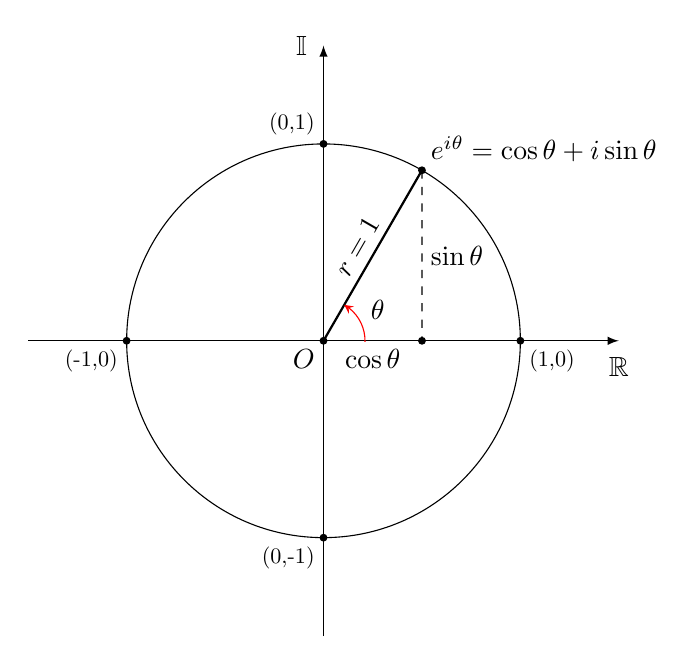
\begin{tikzpicture}[>=stealth, inner sep=3pt,scale=2.5]
      \draw[-latex] (-1.5,0) -- node[below left]{$O$} (1.5,0)
                coordinate[yshift=-0.10cm,label=below:$\mathbb{R}$](x);					% make and label the axes
      \fill[black] (0,0) circle(0.02);                                                  % draw a black dot at the origin
      \draw[-latex] (0,-1.5) -- (0,1.5) node[xshift=-0.10cm, left]{$\mathbb{I}$};
      \draw (0,0) coordinate(o) circle [radius=1cm];                                    % draw unit circle
      \coordinate (p) at (60:1);                                                        % 60 degrees with r = 1
      \fill (p) coordinate[label={above right: ${e^{i\theta} =
                \cos \theta + i \sin \theta}$}] (p) circle(0.02);                       % Euler's formula 
      \coordinate (q) at (p|-o);
%
% draw the various 1s around the unit circle
%
     \coordinate (a) at (0,1);
     \fill (a) coordinate [label={above left: ${\scalebox {0.80}
                          {(0,1)}} $}] (a) circle(0.02);                                % draw coordinates (making them a bit smaller) 
     \coordinate (b) at (-1,0);
     \fill (b) coordinate [label={below left:${\scalebox {0.80}
                          {(-1,0)}}$}] (b) circle(0.02);                                % draw coordinates
     \coordinate (c) at (0,-1);
     \fill (c) coordinate [label={below left:${\scalebox {0.80}
                          {(0,-1)}}$}] (c) circle(0.02);                                % draw coordinates
     \coordinate (d) at (1,0);
     \fill (d) coordinate [label={below right:${\scalebox {0.80}
                          {(1,0)}}$}] (d) circle(0.02);                                 % draw coordinates
%
% do the rest of the labeling and draw the angle
%
     \draw[thick,line join=round] (o) -- node[rotate=60,above]{$r = 1$}(p);             % label r
     \draw [dashed] (p) -- (q) node [midway, right]{${\sin \theta}$}; 
     \draw [] (q) -- (o) node [midway, below] {${\cos \theta}$};        
     \fill (q) coordinate [] (q) circle(0.02);                                          % put a dot at (q)
     \pic[draw=red,"$\theta$",angle radius=15pt,angle
                   eccentricity=1.5,->]{angle=x--o--p};                                 % draw the angle 
    \end{tikzpicture}                                                                   % end tikzpicture
  }                                                                                     % end resizebox
\caption{Euler's Formula, the Unit Circle, and the Complex Plane}
\label{fig:eulers_formula}
\end{figure}


\bigskip
\noindent
There are several ways to derive Euler's formula. One method uses
the Maclaurin series for $\cos \theta$, $\sin \theta$ and
$\mathrm{e}^x$ \cite{wiki:taylor}. To see how this works, notice
that the Maclaurin series for $\cos \theta$ is

\bigskip
\begin{equation}
\cos \theta = 1 - \frac{\theta^2}{2!} + \frac{\theta^4}{4!} - \frac{\theta^6}{6!} + \cdots 
\label{eqn:cos}
\end{equation}

\bigskip
\noindent
while the Maclaurin series for $\sin \theta$ is 

\bigskip
\begin{equation}
\sin \theta = \theta - \frac{\theta^3}{3!} + \frac{\theta^5}{5!} - \frac{\theta^7}{7!} + \cdots 
\label{eqn:sin}
\end{equation}

\bigskip
\noindent
Finally, the Maclaurin series for $\mathrm{e}^x$ is 

\bigskip
\begin{equation}
\mathrm{e}^x = 1 +  x +  \frac{x^2}{2!} + \frac{x^3}{3!} + \frac{x^4}{4!} + \cdots 
\label{eqn:e_to_the_x}
\end{equation}

\medskip
\bigskip
\noindent
Now, if we set $x = i\theta$ in Equation (\ref{eqn:e_to_the_x}) we see that

\bigskip
\begin{equation*}
\begin{array}{lllll}
e^{i\theta}
&=& {\displaystyle 1 + i\theta +  \frac{(i\theta)^2}{2!} +
                   \frac{(i\theta)^3}{3!} + \frac{(i\theta)^4}{4!} +
                   \frac{(i\theta)^5}{5!} + \frac{(i\theta)^6}{6!} +
                   \frac{(i\theta)^7}{7!} + \cdots}    
        &\qquad \mathrel{\#} \text{set $x = i\theta$ in Equation (\ref{eqn:e_to_the_x})}  \\
[13pt]
&=& {\displaystyle 1 +  i\theta -  \frac{\theta^2}{2!} -  \frac{i
                   \theta^3}{3!} + \frac{\theta^4}{4!}  + \frac{i \theta^5}{5!} -
                   \frac{\theta^6}{6!} - \frac{i \theta^7}{7!}  + \cdots}
        &\qquad \mathrel{\#} i^2 = -1, \;  i^3 = -i, \; i^4 = 1, \;  i^5 = i, \; \hdots \\
[12pt]
&=& {\displaystyle \left [ 1 -  \frac{\theta^2}{2!}  +
                   \frac{\theta^4}{4!} - \frac{\theta^6}{6!} + \cdots  \right ]+
                   \left [ i\theta  - \frac{i \theta^3}{3!} + \frac{i \theta^5}{5!}
                   - \frac{i \theta^7}{7!} + \cdots \right ]}                  
        &\qquad \mathrel{\#} \text{group terms} \\
[12pt]
&=& {\displaystyle  \left [ 1 -  \frac{\theta^2}{2!}  +
                    \frac{\theta^4}{4!} - \frac{\theta^6}{6!} +
                    \cdots  \right ]+ i \left [ \theta  -
                    \frac{\theta^3}{3!} + \frac{\theta^5}{5!} -
                    \frac{\theta^7}{7!} + \cdots \right ]}                   
        &\qquad \mathrel{\#} \text{factor out $i$ in the second term} \\
[20pt]
&=& {\displaystyle \cos \theta + i \sin \theta}
        &\qquad \mathrel{\#} \text{Equations (\ref{eqn:cos}) and (\ref{eqn:sin})}
\end{array}
\end{equation*}

\bigskip
\noindent
So we wind up with

\bigskip
\begin{equation}
\mathrm{e}^{i\theta} = \cos \theta + i \sin \theta
\label{eqn:eulers_formula}
\end{equation}

\bigskip
\noindent
that is, Euler's formula.

\subsection{Aside: Why does $e^{2\pi ik} =1$ for $k \in \mathbb{Z}$?}
\label{subsection:e_to_the_2pik_equals_one}

\medskip
Consider the following:

\begin{itemize}
\item {\bf Euler's formula relates the exponential function $e^{ix}$ 
to the sine and cosine functions}

\medskip
The exponential function $e^{ix}$ is connected to $\cos x$ and
$\sin x$ by Euler's formula (Equation (\ref{eqn:eulers_formula})).


\item {\bf Sine and cosine are periodic functions}

\medskip
Both the cosine and sine functions are periodic with a period of 
$2\pi$. This means that $\cos(x+2\pi k) = \cos x$ for $k \in \mathbb{Z}$, 
and $\sin(x+2\pi k) = \sin x$, again for $k \in \mathbb{Z}$.

\item {\bf $e^{2\pi ik}$ is related to the natural log of 1: $e^z = 1 \Rightarrow z = \ln 1$}

\medskip
The exponential function $e^z = 1$ has solutions when
$z = 2\pi i k$ for $k \in \mathbb{Z}$, since 

\smallskip
\begin{equation*}
\begin{array}{lllll}
e^z
&=& e^{2\pi ik} 
		&\hspace{3em} \mathrel{\#} \text{set $z = 2\pi i k$ for $k \in \mathbb{Z}$} \\
[10pt]
&=& \cos(2\pi k) + i\sin(2\pi k) 
		&\hspace{3em} \mathrel{\#} \text{by Euler's formula (Equation (\ref{eqn:eulers_formula}))} \\
[10pt]
&=& 1 + i \cdot 0
		&\hspace{3em} \mathrel{\#} \text{since $\cos(2\pi k) = 1$ and $\sin(2\pi k) = 0$ for $k \in \mathbb{Z}$} \\
[10pt]
&=& 1 
		&\hspace{3em} \mathrel{\#} \text{since $i \cdot 0 = 0$ and $1+0 = 1$} \\
[10pt]
&\Rightarrow& e^{2\pi ik} = 1 
		&\hspace{3em} \mathrel{\#} \text{by the previous lines} \\
[10pt]
&\Rightarrow& e^{z} = 1 
		&\hspace{3em} \mathrel{\#} \text{$z = 2\pi i k$ for $k \in \mathbb{Z}$}

\end{array}
\end{equation*}
\end{itemize}


\medskip
\noindent
So interestingly, the expression $e^{2\pi ik} = 1$ reflects the periodic nature of 
the exponential function in the complex plane. This periodicity is shown in 
Figure \ref{fig:eulers_formula}.


\medskip
\subsection{Deriving Euler's Formula Using Polar Coordinates}
\label{subsec:without_maclaurin0}
There is also a clever way to derive Euler's formula using polar
coordinates. This approach seems to require the fewest
assumptions of the non-Maclaurin series derivations described in
the this and the following sections. To see how this works, first
notice that all non-zero complex numbers can be expressed in
polar coordinates in a unique way. In particular, any number of
the form $e^{ix}$ (with $x \in \mathbb{R}$) which is non-zero can
be expressed as\footnote{Note to self: remember to observe the 
difference between Equation (\ref{eqn:polar}), where $e$ is 
raised to the $ix$ power, and Euler's formula, where $e$ 
is raised to the $i\theta$ power.}


\begin{equation}
e^{ix} = r \left ( \cos \theta + i \sin \theta \right )
\label{eqn:polar}
\end{equation}

\bigskip
\noindent
This is shown in Figure \ref{fig:complex_plane}. In this case $\theta$ 
is the principal angle from the positive real axis (with say, 
$0 \leq \theta \leq 2 \pi$) and $r$ is its radius ($r > 0$). One of the 
features of this proof is that AFAICT it makes no assumption about the 
values of $r$ and $\theta$, except for the fact that they are functions 
of $x$ (we can think of $r$ as shorthand for $r(x)$; likewise $\theta$ 
is shorthand for $\theta(x)$). An interesting problem that has to be 
solved in this proof is what the relationships between $x, r 
\text{ and } \theta$ are. These relationships (and the values of 
$r$ and $\theta$) will be determined in the course of the proof.

\bigskip
\noindent
So to start, what do we know? Well, we know that when $x = 0$ the
left-hand side of Equation (\ref{eqn:polar}) equals $1$, which
implies that $r$ and $\theta$, being functions of $x$, must
satisfy the initial conditions that $r(0) = 1$ and $\theta(0) =
0$ (since $1 = 1 \cdot \left [ \cos \theta(0) + i \sin \theta(0)
\right ] = 1 \cdot \left [ \cos 0 + i \sin 0 \right ] = 1 \cdot
\left [ 1 + i\cdot 0 \right] = 1 \cdot \left [1 + 0 \right ] =
1$).


\bigskip
\noindent
Now, if we differentiate both sides of Equation (\ref{eqn:polar})
with respect to $x$ we see that 


\begin{equation*}
\begin{array}{lllll}
\dfrac{d}{dx} e^{ix} 
&=& \dfrac{d}{dx} \bigg [  r \left ( \cos \theta + i \sin \theta \right ) \bigg ]
                &\mathrel{\#} \text{differentiate both sides with
                respect to $x$}  \\ 
[14pt]
&\Rightarrow& i  e^{ix}  = \dfrac{d}{dx} \bigg [  r \left ( \cos
                \theta + i \sin \theta \right ) \bigg ]
                &\mathrel{\#} \text{apply the chain rule to the LHS}  \\
[14pt]
&\Rightarrow& i  e^{ix}  = \dfrac{dr}{dx}  ( \cos \theta + i
                \sin \theta ) + r \dfrac{d}{dx} \bigg [ \cos
                \theta + i \sin \theta \bigg ] 
                &\mathrel{\#} \text{apply the product rule to the RHS}  \\
[14pt]
&\Rightarrow& i  e^{ix}  = \dfrac{dr}{dx}  ( \cos \theta + i
                \sin \theta ) + r \bigg [\dfrac{d}{dx} \cos \theta +i
                \dfrac{d}{dx} \sin \theta \bigg ]
                &\mathrel{\#} \text{derivative is a linear
                operator \cite{wiki:linearity_of_differentiation}} \\ 
[14pt]
&\Rightarrow& i  e^{ix}  = \dfrac{dr}{dx}  ( \cos \theta + i
                \sin \theta ) + r \bigg [(- \sin \theta) \dfrac{d
                \theta}{dx} + (i \cos \theta) \dfrac{d \theta}{dx} \bigg ]   
                &\mathrel{\#} \dfrac{d}{dx} \cos u = - \sin u
                        \dfrac{du}{dx}, \,  \dfrac{d}{dx} \sin u
                        = \cos u \dfrac{du}{dx}\\  
[14pt]
&\Rightarrow& i  e^{ix}  = \dfrac{dr}{dx}  ( \cos \theta + i
                \sin \theta ) + r (- \sin \theta + i \cos \theta)
                \dfrac{d\theta}{dx} 
                &\mathrel{\#} \text{factor out $\dfrac{d\theta}{dx}$}  \\ 
[14pt]
&\Rightarrow& i  e^{ix}  = ( \cos \theta + i \sin \theta )
                \dfrac{dr}{dx} + r (- \sin \theta + i \cos \theta )
                \dfrac{d\theta}{dx}
                &\mathrel{\#} \text{put the RHS into a more convenient form}
\end{array}
\end{equation*}

\bigskip
\noindent
Note that we are looking for an expression that is unique in
terms of $r$ and $\theta$ so we would like to get rid the
$e^{ix}$ term. One way to do this is to substitute $r (\cos
\theta + i \sin \theta)$ for $e^{ix}$ (Equation (\ref{eqn:polar}))
on the left hand side of the last equation above, which gives us

\begin{equation*}
i r (\cos \theta + i \sin \theta) = (\cos \theta + i \sin \theta)
\dfrac{dr}{dx} + r (-\sin \theta + i \cos \theta) \dfrac{d
\theta}{dx} 
\end{equation*}

\bigskip
\noindent
Multiplying through by $i$ on the left hand side gives

\begin{equation*}
r (i \cos \theta - \sin \theta) = (\cos \theta + i \sin \theta)
\dfrac{dr}{dx} + r (-\sin \theta + i \cos \theta) \dfrac{d
\theta}{dx} 
\end{equation*}

\bigskip
\noindent
and multiplying through on both sides side gives


\begin{equation}
ir \cos \theta -  r \sin \theta = (\cos \theta) \dfrac{dr}{dx} + 
(i \sin \theta) \dfrac{dr}{dx} + (-r \sin \theta) \dfrac{d \theta}{dx}  + 
(i r \cos \theta) \dfrac{d \theta}{dx}
\label{eqn:eqn0}
\end{equation}

\bigskip
\noindent
Next, equating the imaginary and real parts on both sides of
Equation (\ref{eqn:eqn0}) we see that 

\bigskip
\begin{equation*}
ir \cos \theta =  i \sin \theta \dfrac{dr}{dx} +  i r \cos \theta \dfrac{d \theta}{dx}
\end{equation*}

\bigskip
\noindent
and

\begin{equation*}
-  r \sin \theta = \cos \theta \dfrac{dr}{dx} -r \sin \theta \dfrac{d \theta}{dx} 
\end{equation*}

\bigskip
\noindent
Now we have is a system of two equations in two unknowns:
$\dfrac{dr}{dx}$ and $\dfrac{d \theta}{dx}$.  To solve this
system, first assign $\alpha = \dfrac{dr}{dx}$ and $\beta =
\dfrac{d \theta}{dx}$ so that

\bigskip
\begin{equation}
r \cos \theta = (\sin \theta) \alpha + (r \cos \theta) \beta 
\label{eqn:eqn1}
\end{equation}

\bigskip
\noindent
and

\begin{equation}
- r \sin \theta = (\cos \theta) \alpha - (r \sin \theta) \beta 
\label{eqn:eqn2}
\end{equation}

\bigskip
\noindent
Next, by multiplying Equation (\ref{eqn:eqn1}) by $\cos \theta$ and
Equation (\ref{eqn:eqn2}) by $\sin \theta$ we get

\bigskip
\begin{equation}
r \cos^2 \theta = (\sin \theta \cos \theta) \alpha + (r \cos^2 \theta) \beta 
\label{eqn:eqn3}
\end{equation}

\bigskip
\noindent
and

\begin{equation}
- r \sin^2 \theta = (\sin \theta\cos \theta) \alpha - (r \sin^2 \theta) \beta 
\label{eqn:eqn4}
\end{equation}


\bigskip
\noindent
We can eliminate $\alpha$ by subtracting Equation (\ref{eqn:eqn4})
from Equation (\ref{eqn:eqn3}) to get 
 
\medskip
\begin{equation}
r (\cos^2 \theta + \sin^2 \theta)  = r (\cos^2 \theta + \sin^2 \theta)\beta
\label{eqn:eqn5}
\end{equation}

\bigskip
\noindent
and since $\cos^2 \theta + \sin^2 \theta = 1$ Equation
(\ref{eqn:eqn5}) simplifies to  

\medskip
\begin{equation}
r  = r \beta
\label{eqn:eqn6}
\end{equation}

\bigskip
\noindent
Since $r > 0$ for all $x$ Equation (\ref{eqn:eqn6}) tells us that
$\beta$, which we set equal to $\dfrac{d \theta}{dx}$, must equal
1.  If we substitute $\dfrac{d \theta}{dx} = 1$ back into
Equations (\ref{eqn:eqn1}) and (\ref{eqn:eqn2}) we see that


\medskip
\begin{equation*}
\begin{array}{lllll}
& 0 = (\sin \theta) \alpha \\
& 0 =  (\cos \theta) \alpha 
\end{array}
\end{equation*}

\bigskip
{\setstretch{1.5}
\noindent
which implies that $\alpha \sin \theta = \alpha \cos \theta$
which in turn implies that $\alpha = 0$. But why does $\alpha =
0$? One way to think about this is to consider that $\alpha \sin
\theta = \alpha \cos \theta \Rightarrow \dfrac{\sin \theta}{\cos
\theta} = \tan \theta = 1$.  This occurs when $\theta =
\dfrac{\pi}{4} + n \pi$ for $n \in \mathbb{Z}$. Since neither
$\sin \theta$ nor $\cos \theta$ equals zero for these values of
$\theta$ we can conclude that $\alpha$ must equal zero. \par}


\bigskip
\noindent
Now, recall that $\alpha = \dfrac{dr}{dx}$ so now we know that
$\dfrac{dr}{dx} = 0$ and $\dfrac{dr}{dx} = 0 \Rightarrow r(x) =
a$ for some constant $a$.  Similarly, since $\dfrac{d\theta}{dx}
= 1$ we know that $d \theta = dx$ and integrating both sides we
see that

\bigskip
\begin{equation}
\int d \theta  = \int dx \Rightarrow \theta(x) = x + C
\label{eqn:int}
\end{equation}

\bigskip
\noindent
for some constant $C$.

\bigskip
\noindent
Going back to the very beginning where we saw that $r(0) = 1$ and
since we know that $r(x) = a$ for all $x$, $r$ must equal 1 for
all $x$. Similarly because $\theta(0) = 0$ we see that $\theta(0)
= 0 + C$ (Equation (\ref{eqn:int})), so it must be that $C$ equals
zero. Said another way, now we know that $\theta(x) = x$ or more
concisely, $\theta = x$.

\bigskip
\noindent
So $r = 1$ and $\theta = x$. Substituting these values back into
Equation (\ref{eqn:polar}) we see that  

\bigskip
\begin{equation*}
\begin{array}{lllll}
e^{ix} 
&=& r \cdot \left [ \cos \theta + i \sin \theta \right ]
		&\qquad \qquad \qquad \qquad \mathrel{\#} \text{Equation (\ref{eqn:polar})} \\
[8pt]
&=& 1 \cdot \left [ \cos x + i \sin x \right ]
		&\qquad \qquad \qquad \qquad \mathrel{\#} \text{$r = 1$ and $\theta = x$} \\
[8pt]
&=& \cos x + i \sin x
		&\qquad \qquad \qquad \qquad \mathrel{\#} \text{Euler's formula}
\end{array}
\end{equation*}


\medskip
\subsection{Another Approach To Euler's Formula Without Maclaurin Series}
\label{subsec:without_maclaurin1}
A different way to derive Euler's formula without using Maclaurin
series starts by defining  

\bigskip
\begin{equation*}
f(\theta) = e^{-i\theta} \left ( \cos \theta + i\sin \theta \right )
\end{equation*}

\bigskip
\noindent
for all real $\theta$. Then 


\begin{equation*}
\begin{array}{lllll}
f(\theta)
&=&  e^{-i\theta} \left ( \cos \theta + i\sin \theta \right)                                                                                                  		&\mathrel{\#} \text{definition of $f(\theta)$} \\
[10pt]
&\Rightarrow& f^{\prime}(\theta)  = \dfrac{d}{d \theta} 
	\Big [ e^{-i\theta} \left ( \cos \theta + i\sin \theta \right) \Big ]     
		&\mathrel{\#}  \text{take derivative of both sides} \\
[14pt]
&\Rightarrow& f^{\prime}(\theta)  = e^{-i\theta} \cdot  \dfrac{d}{d\theta}  
	(\cos \theta +i \sin \theta)+ \dfrac{d}{d\theta} e^{-i\theta} (\cos \theta + i\sin \theta )                                        
		&\mathrel{\#}  \text{product rule} \\
[14pt]
&\Rightarrow& f^{\prime}(\theta)  = e^{-i\theta }(i\cos \theta -\sin \theta ) + 
	\dfrac{d}{d\theta} e^{-i\theta} (\cos \theta + i\sin \theta )
		&\mathrel{\#}  \dfrac{d}{d\theta}  (\cos \theta +i \sin \theta) = i\cos \theta -\sin \theta \\
[14pt]
&\Rightarrow& f^{\prime}(\theta)  = e^{-i\theta }(i\cos \theta -\sin \theta ) + 
	ie^{-i\theta} (\cos \theta + i\sin \theta )
		&\mathrel{\#} \text{chain rule} \\
[14pt]
&\Rightarrow&f^{\prime}(\theta) = e^{-i\theta} \cdot \Big [ (i\cos \theta -\sin \theta) - 
	i (\cos \theta +i\sin \theta)  \Big ]  
		&\mathrel{\#} \text{factor out $e^{-i\theta}$} \\
[14pt]
&\Rightarrow&f^{\prime}(\theta) = e^{-i\theta} \cdot \Big [ (i\cos \theta -\sin \theta) -  
	(i\cos \theta -\sin \theta)  \Big ]
		&\mathrel{\#} \text{multiply through by $i$} \\
[14pt]
&\Rightarrow&f^{\prime}(\theta) = e^{-i\theta} \cdot 0                                                                                                     		&\mathrel{\#} \Big [ (i\cos \theta -\sin \theta) -  
			(i\cos \theta -\sin \theta)  \Big ]  = 0 \\
[14pt]
&\Rightarrow&f^{\prime}(\theta) =  0                                                                                                                               		&\mathrel{\#} \text{simplify}
\end{array}
\end{equation*}

\bigskip
\noindent
Since $f^{\prime}(\theta) = 0$ we know that $f(\theta)$ is a
constant (that is, $f(x) = a$ for some constant $a$). We also
know that  

\medskip
\begin{equation*}
f(0) = e^{-i0} \cdot \big [\cos 0 + i \sin 0 \big ]  
     = 1 \cdot \big [1 + 0 \big ] = 1
\end{equation*}

\medskip
\bigskip
\noindent
Now, since $f(\theta)$ is a constant and $f(0) = 1$ we know that
$f(\theta) = 1$ for all real $\theta$.  Dividing both sides by
$e^{-i\theta}$ yields

\bigskip
\begin{equation*}
\dfrac{f(\theta)}{e^{-i\theta}} = \dfrac{1}{e^{-i\theta}} =
\dfrac{e^{-i\theta} \cdot (\cos \theta + i \sin
\theta)}{e^{-i\theta}} 
\end{equation*}

\medskip
\bigskip
\noindent
and we wind up with Euler's formula: $e^{i\theta }=\cos \theta
+i\sin \theta$ 


\bigskip
\subsection{One More Approach To Euler's Formula}
\label{subsec:without_maclaurin2}
Finally, while the approach in this section is similar to the
approach proposed in Section \ref{subsec:without_maclaurin1},
some people prefer this approach as it seems to require fewer
assumptions (as I mentioned above, the approach taken in Section
\ref{subsec:without_maclaurin0} seems to require the fewest
assumptions). In any event, the proof goes as follows:


\medskip
\begin{equation*}
\begin{array}{lllll}
z
&=& \cos{\theta}+i\sin{\theta}
                &\qquad \mathrel{\#} \text{definition of a
                complex number (Figure \ref{fig:complex_plane})} \\ 
[12pt]
&\Rightarrow& \dfrac{dz}{d\theta} = \dfrac{d}{d \theta} 
	\left [ \cos{\theta}+i\sin{\theta}  \right ]
                &\qquad \mathrel{\#} \text{take the derivative of
                both sides} \\ 
[14pt]
&\Rightarrow& \dfrac{dz}{d\theta} = \dfrac{d}{d \theta} \cos{\theta} + 
	\dfrac{d}{d \theta} i\sin{\theta}
                &\qquad \mathrel{\#} \text{derivative is a linear
                operator} \\ 
[14pt]
&\Rightarrow& \dfrac{dz}{d\theta} =- \sin{\theta} + i\cos{\theta}
                &\qquad \mathrel{\#} \text{$ \dfrac{d}{d \theta}
                \cos{\theta} = - \sin \theta$ and $\dfrac{d}{d
                \theta} i\sin{\theta} =  i\cos{\theta}$} \\ 
[14pt]
&\Rightarrow& \dfrac{dz}{d\theta} = iz
                &\qquad \mathrel{\#}  i z  = i \left [
                \cos{\theta}+i\sin{\theta}  \right ] =
                -\sin{\theta} + i\cos{\theta} \\
\end{array}
\end{equation*}

\bigskip
\noindent
So now we know that $\dfrac{dz}{d\theta} = iz$, which implies
that $\dfrac{dz}{z} = i \, d\theta$. This means that 

\bigskip
\begin{equation*}
\begin{array}{lllll}
\dfrac{dz}{z} 
&=& {\displaystyle  i \, d\theta}
                &\qquad \mathrel{\#} \text{result from above} \\
[12pt]
&\Rightarrow& {\displaystyle \int \frac{dz}{z} =  \int i \,
d\theta}
                &\qquad \mathrel{\#} \text{integrate both sides} \\
[12pt]
&\Rightarrow&  {\displaystyle \ln{|z|} = i \theta + C}
                &\qquad \mathrel{\#} \text{${\displaystyle \int
                \frac{dz}{z} =  \ln{|z|}}$ and ${\displaystyle
                \int i \: d\theta = {i \, \theta +C}}$} \\ 
[12pt]
&\Rightarrow&  {\displaystyle z = e^{i\theta +C}}
                &\qquad \mathrel{\#} \text{exponentiate both
                sides: $e^{\ln |z|} = z$ and $e^{i \theta +C} =
                e^{i \theta +C}$}
\end{array}
\end{equation*}

\bigskip
\noindent
Now, we know $z(0) = \cos 0 + i \sin 0 = 1 + i \cdot 0 =1$. We
also know that $z(0) = e^{0i +C} = e^{C} = 1$. Since $e^{C} = 1$
we know that $C$ must equal $0$. Putting all of this together we
see that $z = e^{i\theta}=\cos{\theta}+i\sin{\theta}$, that is,
Euler's formula.


\bigskip
\section{Euler's Identity}
Something interesting happens when we set $\theta = \pi$ in
Euler's formula. We get Euler's identity \cite{wiki:eulers_identity}.

\bigskip
\begin{equation*}
\begin{array}{lllll}
e^{i\theta}
&=& \cos \theta + i \sin \theta                         
	&\qquad \qquad \qquad \qquad  \mathrel{\#} \text{Euler's formula (Equation (\ref{eqn:eulers_formula}))} \\
[5pt]
&\Rightarrow&  e^{i\pi} = \cos \pi + i \sin \pi         
	&\qquad \qquad \qquad \qquad  \mathrel{\#} \text{set $\theta = \pi$} \\
[5pt]
&\Rightarrow&  e^{i\pi} = -1 + i \cdot 0                
	&\qquad \qquad \qquad \qquad  \mathrel{\#} \text{$\cos \pi = -1$ and $\sin \pi = 0$} \\
[5pt]
&\Rightarrow&  e^{i\pi} = -1 + 0                        
	&\qquad \qquad \qquad \qquad  \mathrel{\#} i \cdot 0 = 0 \\
[5pt]
&\Rightarrow&  e^{i\pi} = -1                            
	&\qquad \qquad \qquad \qquad  \mathrel{\#} \text{simplify} \\
[5pt]
&\Rightarrow&  e^{i\pi} +1 = 0                          
	&\qquad \qquad \qquad \qquad  \mathrel{\#} \text{Euler's identity} 
\end{array}
\end{equation*}
%
%
%
\bigskip
\section{Conclusions}
%
%
%
\bigskip
\section{Acknowledgements}
Thanks to Dave Neary for suggesting a non-Maclaurin series 
derivation of Euler's formula and encouraging my study of 
the non-Maclaurin series derivations of Euler's formula.
%
%	LaTeX source on overleaf.com
%
\section*{\LaTeX \hspace{0.10 mm} Source}
\url{https://www.overleaf.com/read/gczxmjgfrxxb}
%
%	get a bibliography
%
%	Note:.bib files go in ~/Library/texmf/bibtex/bib with TeXShop (MacTeX).
%	You can also use an absolute path, e.g. \bibliography{/Users/dmm/papers/bib/qc}
%
\bibliographystyle{plain}
\bibliography{qc}
%
%	done
%
\end{document} 


